\documentclass[aspectratio=169,10pt]{beamer}
\usepackage[utf8]{inputenc}
\usepackage{tikz}
\usetikzlibrary{shapes.geometric, arrows, positioning, fit, calc}
\usepackage{tcolorbox}
\usepackage{array}
\usepackage{colortbl}
\usepackage{hyperref}
\usepackage{graphicx}
\usepackage{amsmath}
\usepackage{amssymb}

% ==========================================
% CUSTOM DARK COLOR PALETTE (Cyber Dashboard)
% ==========================================
\definecolor{darkbg}{HTML}{0D1117}
\definecolor{panelbg}{HTML}{161B22}
\definecolor{bordercolor}{HTML}{30363D}
\definecolor{critred}{HTML}{F85149}
\definecolor{highamber}{HTML}{FFA657}
\definecolor{modblue}{HTML}{58A6FF}
\definecolor{lowgreen}{HTML}{3FB950}
\definecolor{textwhite}{HTML}{E6EDF3}
\definecolor{textgray}{HTML}{8B949E}
\definecolor{cybercyan}{HTML}{79C0FF}
\definecolor{cyberpurple}{HTML}{D2A8FF}

% ==========================================
% BEAMER STYLING
% ==========================================
\setbeamercolor{background canvas}{bg=darkbg}
\setbeamercolor{normal text}{fg=textwhite}
\setbeamercolor{frametitle}{fg=modblue}
\setbeamerfont{frametitle}{size=\large, series=\bfseries}
\setbeamercolor{title}{fg=modblue}
\setbeamerfont{title}{size=\Huge, series=\bfseries}
\setbeamercolor{subtitle}{fg=textgray}
\setbeamercolor{author}{fg=textwhite}
\setbeamercolor{date}{fg=textgray}
\setbeamercolor{structure}{fg=modblue}

% Remove default navigation symbols
\setbeamertemplate{navigation symbols}{}

% Custom Footer
\setbeamertemplate{footline}{
    \ifnum\insertframenumber>1
        \begin{beamercolorbox}[wd=\paperwidth, ht=3.5ex, dp=1.5ex, leftskip=3ex, rightskip=3ex]{footline}
            \color{textgray}\tiny
            Nitesh Solanki (IIIT Bhopal) \hfill Gridlock Hackathon 2.0 -- Prototype Round \hfill Slide \insertframenumber{} / \inserttotalframenumber
        \end{beamercolorbox}
    \fi
}

% Custom Block Styles
\setbeamercolor{block title}{bg=panelbg, fg=modblue}
\setbeamercolor{block body}{bg=panelbg, fg=textwhite}

% ==========================================
% TCOLORBOX CONFIGURATION FOR DASHBOARD CARDS
% ==========================================
\tcbset{
    dashboardcard/.style={
        colback=panelbg,
        colframe=bordercolor,
        coltext=textwhite,
        arc=4pt,
        boxrule=0.8pt,
        valign=center,
        fonttitle=\bfseries\scriptsize,
        coltitle=modblue,
        left=6pt, right=6pt, top=6pt, bottom=6pt
    },
    metriccard/.style={
        colback=panelbg,
        colframe=bordercolor,
        coltext=textwhite,
        arc=4pt,
        boxrule=1.2pt,
        halign=center,
        valign=center,
        left=4pt, right=4pt, top=4pt, bottom=4pt
    }
}

% ==========================================
% PRESENTATION DOCUMENT
% ==========================================
\begin{document}

% ------------------------------------------
% SLIDE 1: Title Slide (Dashboard Widescreen)
% ------------------------------------------
{
\setbeamertemplate{footline}{} % Hide footer on title slide
\begin{frame}[plain]
    \begin{tikzpicture}[remember picture, overlay]
        % Dark Background
        \fill[color=darkbg] (current picture.south west) rectangle (current picture.north east);
        
        % Right side screenshot backdrop
        \node[anchor=east, opacity=0.3] at ($(current picture.east) + (0.5, -0.5)$) {
            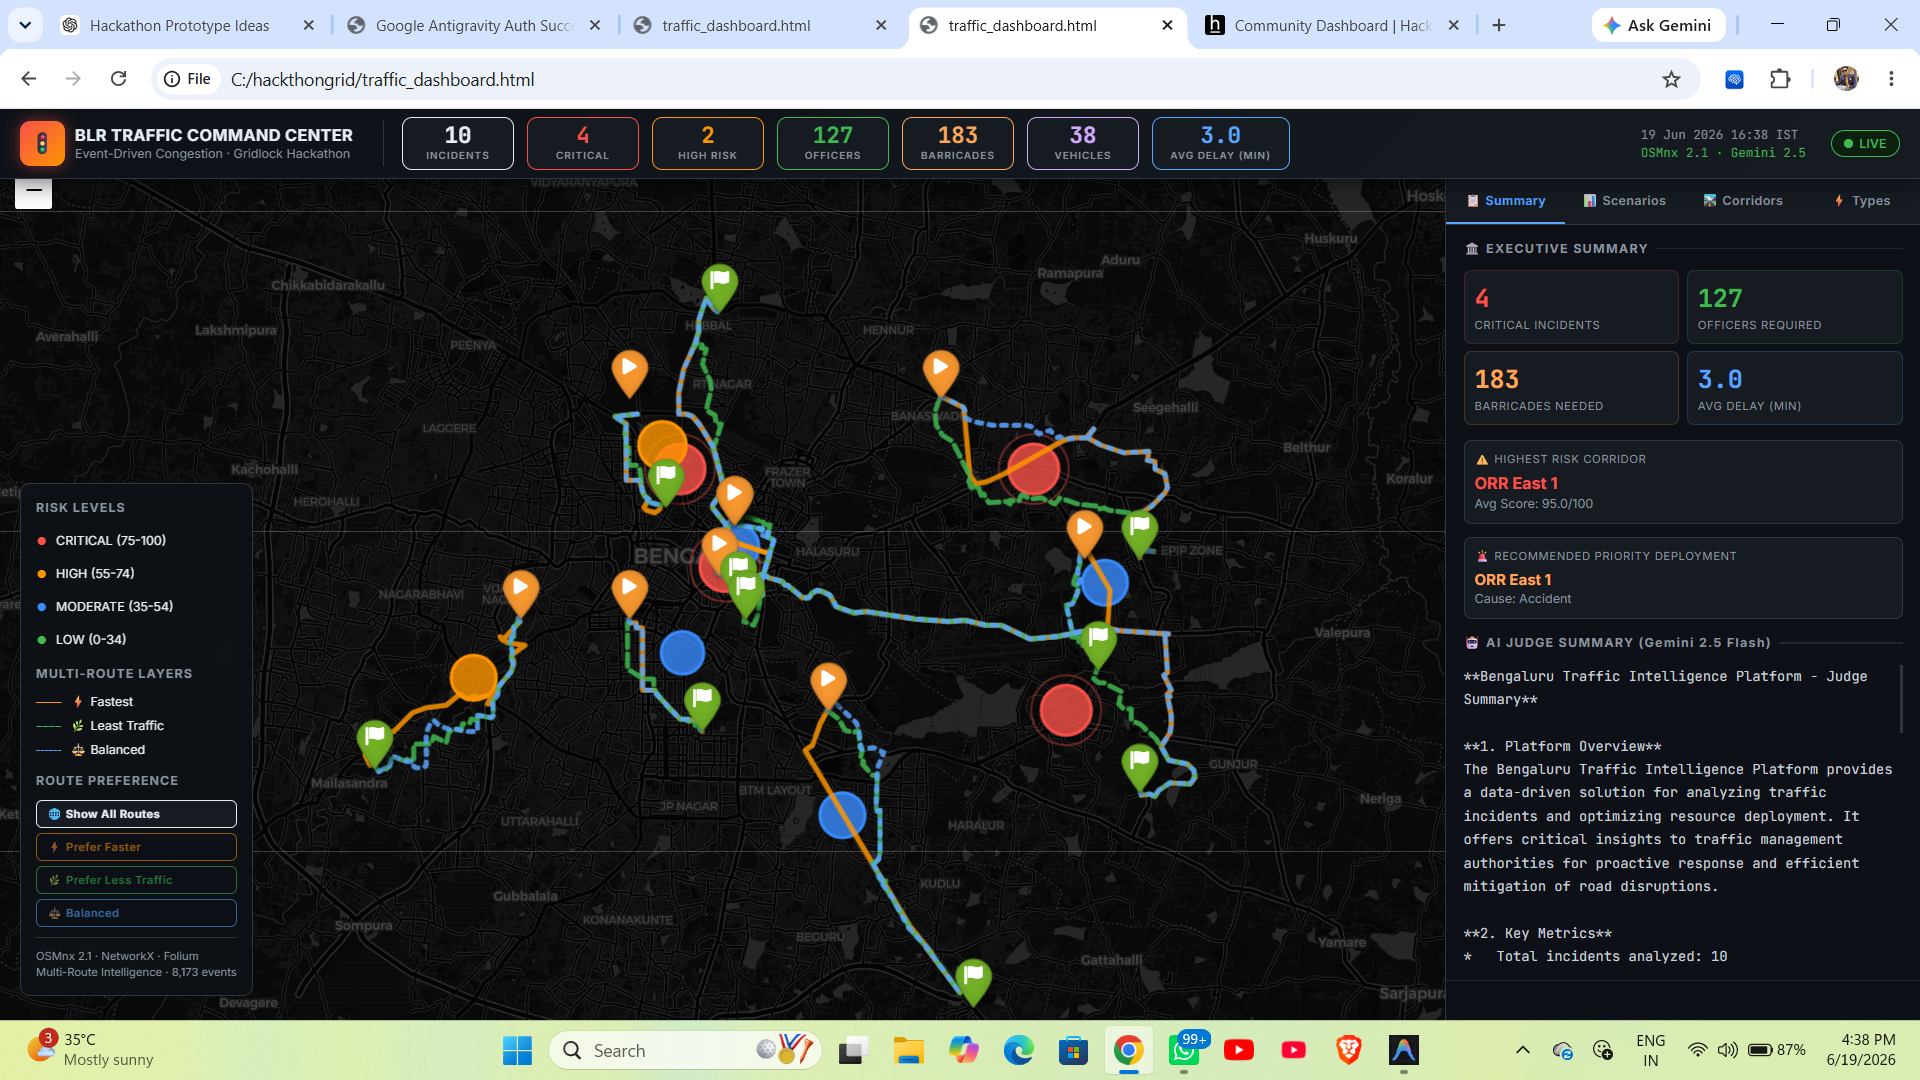
\includegraphics[width=0.55\paperwidth]{presentation_assets/Screenshot (1199).png}
        };
        
        % Left side title details
        \node[anchor=west, text width=0.5\paperwidth] at ($(current picture.west) + (1.0, 0.5)$) {
            {\color{critred}\bfseries\small \textbullet\ LIVE MONITORING ACTIVE}\\[0.3cm]
            {\Huge\color{modblue}\bfseries BLR Traffic\\Command Center}\\[0.4cm]
            {\normalsize\color{textwhite} AI-Powered Event-Driven Traffic Intelligence}\\[0.2cm]
            {\scriptsize\color{textgray} Real-Time Congestion Scoring, Routing \& Resource Management}\\
            \vspace{0.8cm]
            \hrule height 0.5pt color bordercolor\\[0.3cm]
            {\scriptsize\color{textwhite} \textbf{Hackathon:} Gridlock Hackathon 2.0 -- Prototype Round}\\
            {\scriptsize\color{textwhite} \textbf{Developer:} Nitesh Solanki (IIIT Bhopal)}\\
        };
        
        % Bottom glowing accent
        \fill[color=modblue, opacity=0.15] ($(current picture.south west)$) rectangle ($(current picture.south east) + (0, 0.1)$);
    \end{tikzpicture}
\end{frame}
}

% ------------------------------------------
% SLIDE 2: Problem Statement
% ------------------------------------------
\begin{frame}{Problem Statement: Traffic Authorities Are Reactive, Not Predictive}
    \begin{columns}[T]
        \begin{column}{0.48\textwidth}
            \begin{tcolorbox}[dashboardcard, title=THE CORE CHALLENGE, height=0.75\paperheight]
                \color{textwhite}\small
                Modern city traffic management systems rely on cameras and manual reporting, leading to high latency in dispatching support.
                \vspace{0.3cm]
                \begin{itemize}
                    \item \textbf{Spreading Congestion}: Bottlenecks propagate through the road grid before physical intervention can occur.
                    \item \textbf{Manual Resource Allocation}: Police and barricades are deployed based on ad-hoc protocols rather than quantitative demand.
                    \item \textbf{No Active Diversions}: Commuters enter blockages blindly due to lack of dynamic alternative routing.
                    \item \textbf{Informational Silos}: GIS, sensor, and municipal data are rarely unified into actionable command summaries.
                \end{itemize}
            \end{tcolorbox}
        \end{column}
        
        \begin{column}{0.48\textwidth}
            \begin{tcolorbox}[dashboardcard, title=CONGESTION CASCADE TIMELINE, height=0.75\paperheight]
                \centering
                \vspace{0.1cm}
                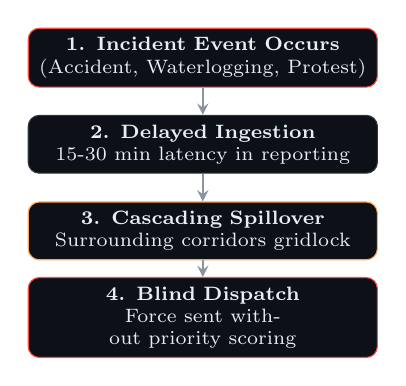
\begin{tikzpicture}[node distance=1.0cm, auto, >=latex']
                    \tikzstyle{box} = [rectangle, draw=bordercolor, fill=darkbg, text=textwhite, rounded corners, minimum width=4cm, minimum height=0.7cm, text width=4.2cm, align=center, font=\scriptsize]
                    \tikzstyle{arrow} = [thick, ->, >=stealth, color=textgray]
                    
                    \node (step1) [box, draw=critred] {\textbf{1. Incident Event Occurs} \\ (Accident, Waterlogging, Protest)};
                    \node (step2) [box, below of=step1, node distance=1.1cm] {\textbf{2. Delayed Ingestion} \\ 15-30 min latency in reporting};
                    \node (step3) [box, below of=step2, node distance=1.1cm, draw=highamber] {\textbf{3. Cascading Spillover} \\ Surrounding corridors gridlock};
                    \node (step4) [box, below of=step3, node distance=1.1cm, draw=critred] {\textbf{4. Blind Dispatch} \\ Force sent without priority scoring};
                    
                    \draw [arrow] (step1) -- (step2);
                    \draw [arrow] (step2) -- (step3);
                    \draw [arrow] (step3) -- (step4);
                \end{tikzpicture}
            \end{tcolorbox}
        \end{column}
    \end{columns}
\end{frame}

% ------------------------------------------
% SLIDE 3: Our Solution
% ------------------------------------------
\begin{frame}{Our Solution: End-to-End Traffic Intelligence System}
    \begin{tcolorbox}[dashboardcard, title=FUNCTIONAL ARCHITECTURE FLOW]
        \centering
        \vspace{0.1cm}
        \begin{tikzpicture}[node distance=1.8cm, auto, >=latex']
            \tikzstyle{block} = [draw=bordercolor, fill=panelbg, text=textwhite, rect, minimum width=2.1cm, minimum height=1.0cm, text width=1.9cm, align=center, font=\scriptsize\bfseries, rounded corners]
            \tikzstyle{highlight} = [draw=modblue, fill=darkbg, text=textwhite, rect, minimum width=2.1cm, minimum height=1.0cm, text width=1.9cm, align=center, font=\scriptsize\bfseries, rounded corners, line width=1pt]
            \tikzstyle{arrow} = [thick, ->, >=stealth, color=textgray]
            
            \node (n1) [block] {1. Event\\Sources};
            \node (n2) [block, right of=n1, node distance=2.4cm] {2. Incident\\Intelligence};
            \node (n3) [highlight, right of=n2, node distance=2.4cm, draw=highamber] {3. Congestion\\Scoring Engine};
            \node (n4) [block, right of=n3, node distance=2.4cm] {4. Resource\\Planner};
            \node (n5) [highlight, right of=n4, node distance=2.4cm, draw=lowgreen] {5. Route\\Optimization};
            \node (n6) [block, right of=n5, node distance=2.4cm] {6. Command\\Dashboard};
            
            \draw [arrow] (n1) -- (n2);
            \draw [arrow] (n2) -- (n3);
            \draw [arrow] (n3) -- (n4);
            \draw [arrow] (n4) -- (n5);
            \draw [arrow] (n5) -- (n6);
        \end{tikzpicture}
    \end{tcolorbox}
    
    \vspace{-0.1cm}
    \begin{columns}[T]
        \begin{column}{0.24\textwidth}
            \begin{tcolorbox}[dashboardcard, title=PREDICT, colframe=critred]
                \scriptsize Detects traffic disruptions and calculates geographical impact radius (1.7 - 4.1 km) before delay loops form.
            \end{tcolorbox}
        \end{column}
        \begin{column}{0.24\textwidth}
            \begin{tcolorbox}[dashboardcard, title=PRIORITIZE, colframe=highamber]
                \scriptsize Dynamic multi-factor engine scores events (0-100) based on severity, rush-hour, and corridor weight.
            \end{tcolorbox}
        \end{column}
        \begin{column}{0.24\textwidth}
            \begin{tcolorbox}[dashboardcard, title=DEPLOY, colframe=cybercyan]
                \scriptsize Recommends exact dispatch numbers (Officers, Barricades, Patrol) matched to the incident cause.
            \end{tcolorbox>
        \end{column}
        \begin{column}{0.24\textwidth}
            \begin{tcolorbox}[dashboardcard, title=DIVERT, colframe=lowgreen]
                \scriptsize Computes secondary sub-graphs over OSMnx to build real alternate routes, bypassing blockages.
            \end{tcolorbox}
        \end{column}
    \end{columns}
\end{frame}

% ------------------------------------------
% SLIDE 4: Platform Overview
% ------------------------------------------
\begin{frame}{Platform Overview: Live Command Center Interface}
    \begin{columns}[T]
        \begin{column}{0.65\textwidth}
            \begin{tcolorbox}[dashboardcard, title=COMMAND CENTER MAIN UI, left=2pt, right=2pt, top=2pt, bottom=2pt]
                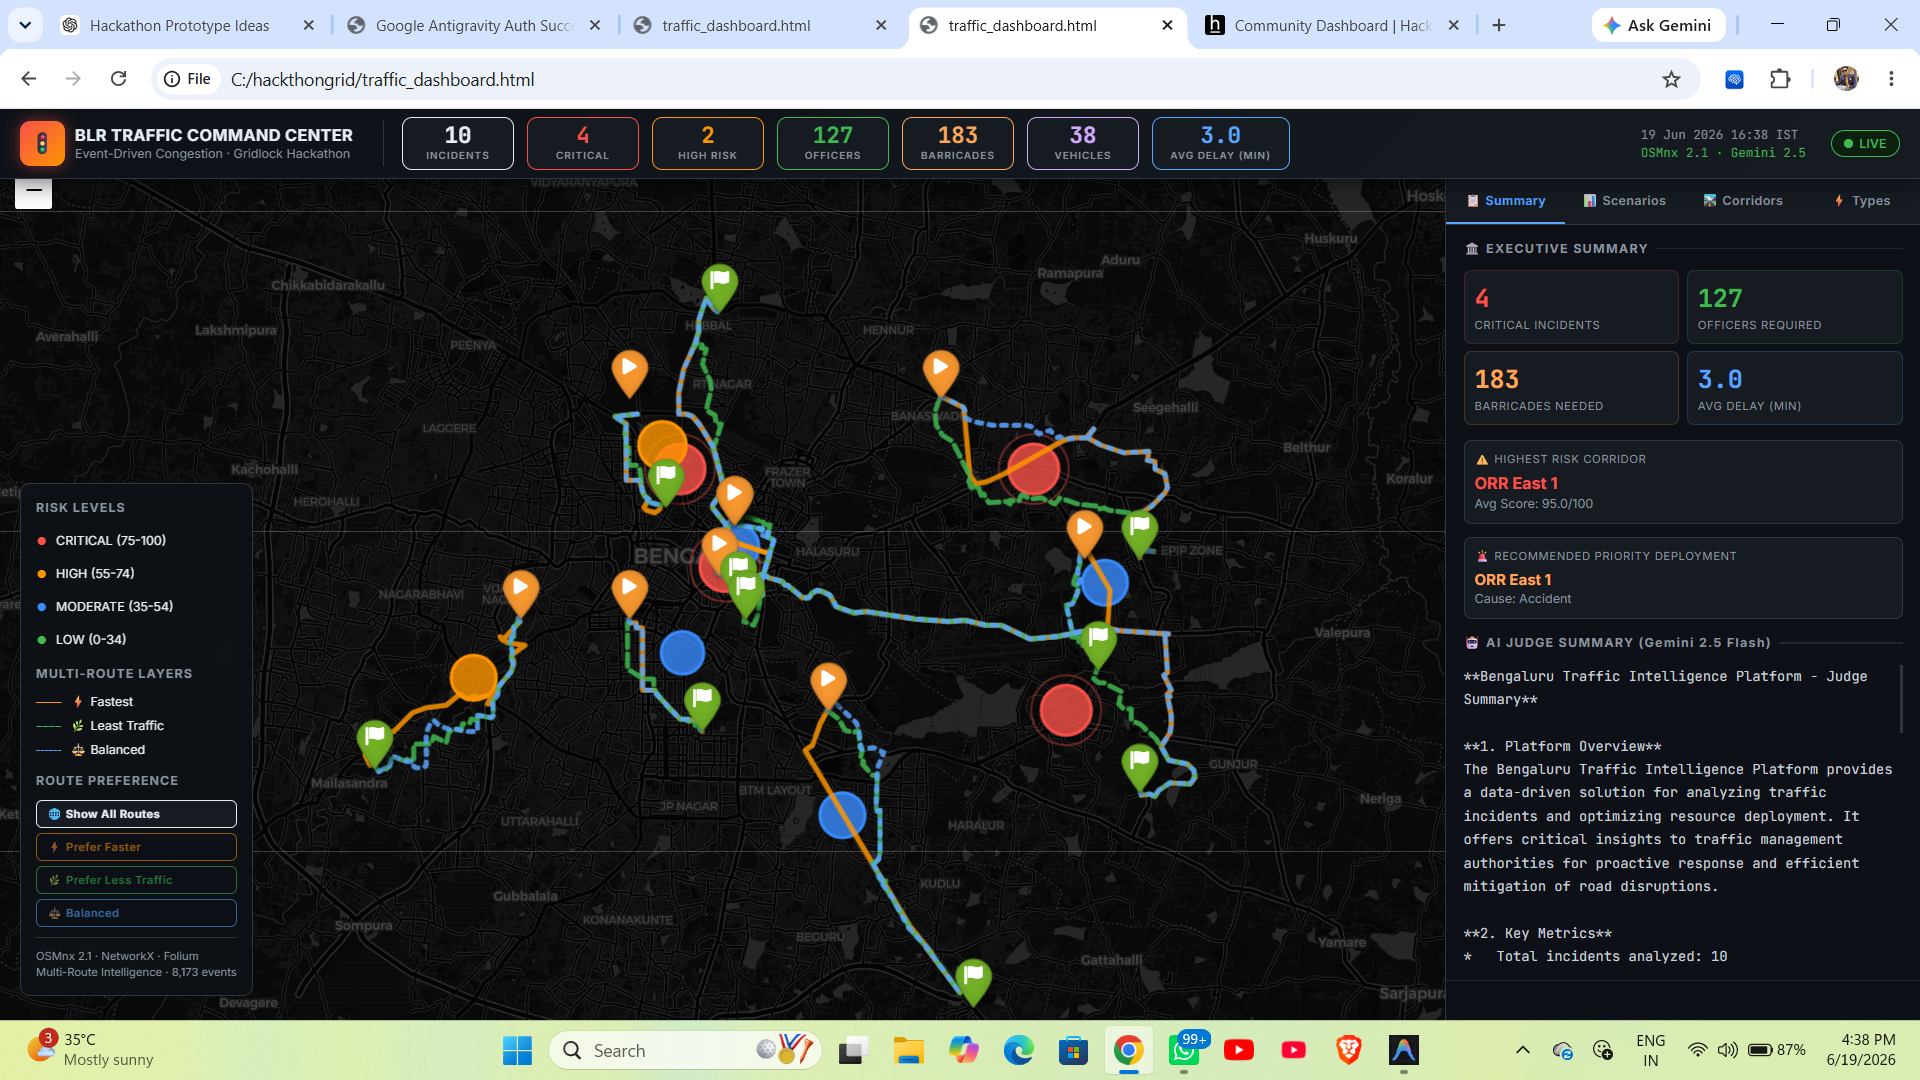
\includegraphics[width=\linewidth]{presentation_assets/Screenshot (1199).png}
            \end{tcolorbox}
            \centering\color{textgray}\tiny ``City-wide operational traffic intelligence dashboard.''
        \end{column}
        
        \begin{column}{0.31\textwidth}
            \begin{tcolorbox}[dashboardcard, title=INTELLIGENT UI LAYER, height=0.75\paperheight]
                \color{textwhite}\scriptsize
                A single unified GIS panel rendering road layers, active metrics, and alternate routes.
                \vspace{0.2cm]
                \begin{itemize}
                    \item \textbf{\color{modblue}Incident Detection}: Interactive circle markers scale dynamically with coordinates.
                    \item \textbf{\color{critred}Risk Triage}: Incidents classified in 4 colors (Critical, High, Moderate, Low).
                    \item \textbf{\color{cybercyan}Route Visualization}: Original path highlighted in Red; bypass routes highlighted in Green.
                    \item \textbf{\color{lowgreen}Resource Overlay}: Renders officer and asset needs directly in the map popup.
                    \item \textbf{\color{cyberpurple}Global Statistics}: Command bar summarizes city-wide demand.
                \end{itemize}
            \end{tcolorbox}
        \end{column}
    \end{columns}
\end{frame}

% ------------------------------------------
% SLIDE 5: System Architecture
% ------------------------------------------
\begin{frame}{System Architecture: Multi-Layer Processing Pipeline}
    \centering
    \begin{tikzpicture}[node distance=1.0cm, auto, >=latex']
        % Style Definitions
        \tikzstyle{layer} = [rectangle, draw=bordercolor, fill=panelbg, text=textwhite, minimum width=13.0cm, minimum height=0.8cm, text width=12.8cm, align=left, font=\scriptsize, rounded corners]
        \tikzstyle{layerlabel} = [font=\tiny\bfseries, color=modblue, fill=panelbg, inner sep=2pt]
        
        % Architecture Stack
        \node (layer5) [layer, draw=cyberpurple] {\textbf{5. GENERATIVE AI LAYER} \\ \quad \textbullet\ Gemini 2.5 Flash API \quad \textbullet\ Automated executive summaries \quad \textbullet\ Plain-text situational briefings};
        
        \node (layer4) [layer, below of=layer5, node distance=1.1cm, draw=lowgreen] {\textbf{4. VISUALIZATION LAYER} \\ \quad \textbullet\ Interactive Folium/Leaflet Map \quad \textbullet\ Metric KPI command bar \quad \textbullet\ Dynamic Javascript popups};
        
        \node (layer3) [layer, below of=layer4, node distance=1.1cm, draw=cybercyan] {\textbf{3. DECISION LAYER (Policy \& Command)} \\ \quad \textbullet\ OSMnx Alternate routing (Dijkstra bypass) \quad \textbullet\ Asset allocator (Officers, Barricades, Vehicles)};
        
        \node (layer2) [layer, below of=layer3, node distance=1.1cm, draw=highamber] {\textbf{2. PROCESSING LAYER (Scoring \& Analytics)} \\ \quad \textbullet\ Congestion Risk Engine (0-100 scale) \quad \textbullet\ Space-Time Indexer (Peak & Rush hour analysis)};
        
        \node (layer1) [layer, below of=layer2, node distance=1.1cm] {\textbf{1. DATA LAYER (Storage \& Ingestion)} \\ \quad \textbullet\ Astram event logs (8,173 clean rows) \quad \textbullet\ OpenStreetMap spatial graphs \quad \textbullet\ Scenario parameters};
        
        % Connective arrow
        \draw[<->, >=stealth, thick, color=textgray] ($(layer1.west) - (0.3, 0)$) -- ($(layer5.west) - (0.3, 0)$) node[midway, left, font=\tiny, text width=1.5cm, align=center] {Bidirectional \\ Pipeline};
    \end{tikzpicture}
\end{frame}

% ------------------------------------------
% SLIDE 6: Incident Intelligence Engine
% ------------------------------------------
\begin{frame}{Incident Intelligence: Multi-Scenario Analysis}
    \begin{columns}[T]
        \begin{column}{0.65\textwidth}
            \begin{columns}
                \begin{column}{0.5\textwidth}
                    \begin{tcolorbox}[dashboardcard, title=ACCIDENT (CRITICAL), colframe=critred, left=1pt, right=1pt, top=1pt, bottom=1pt]
                        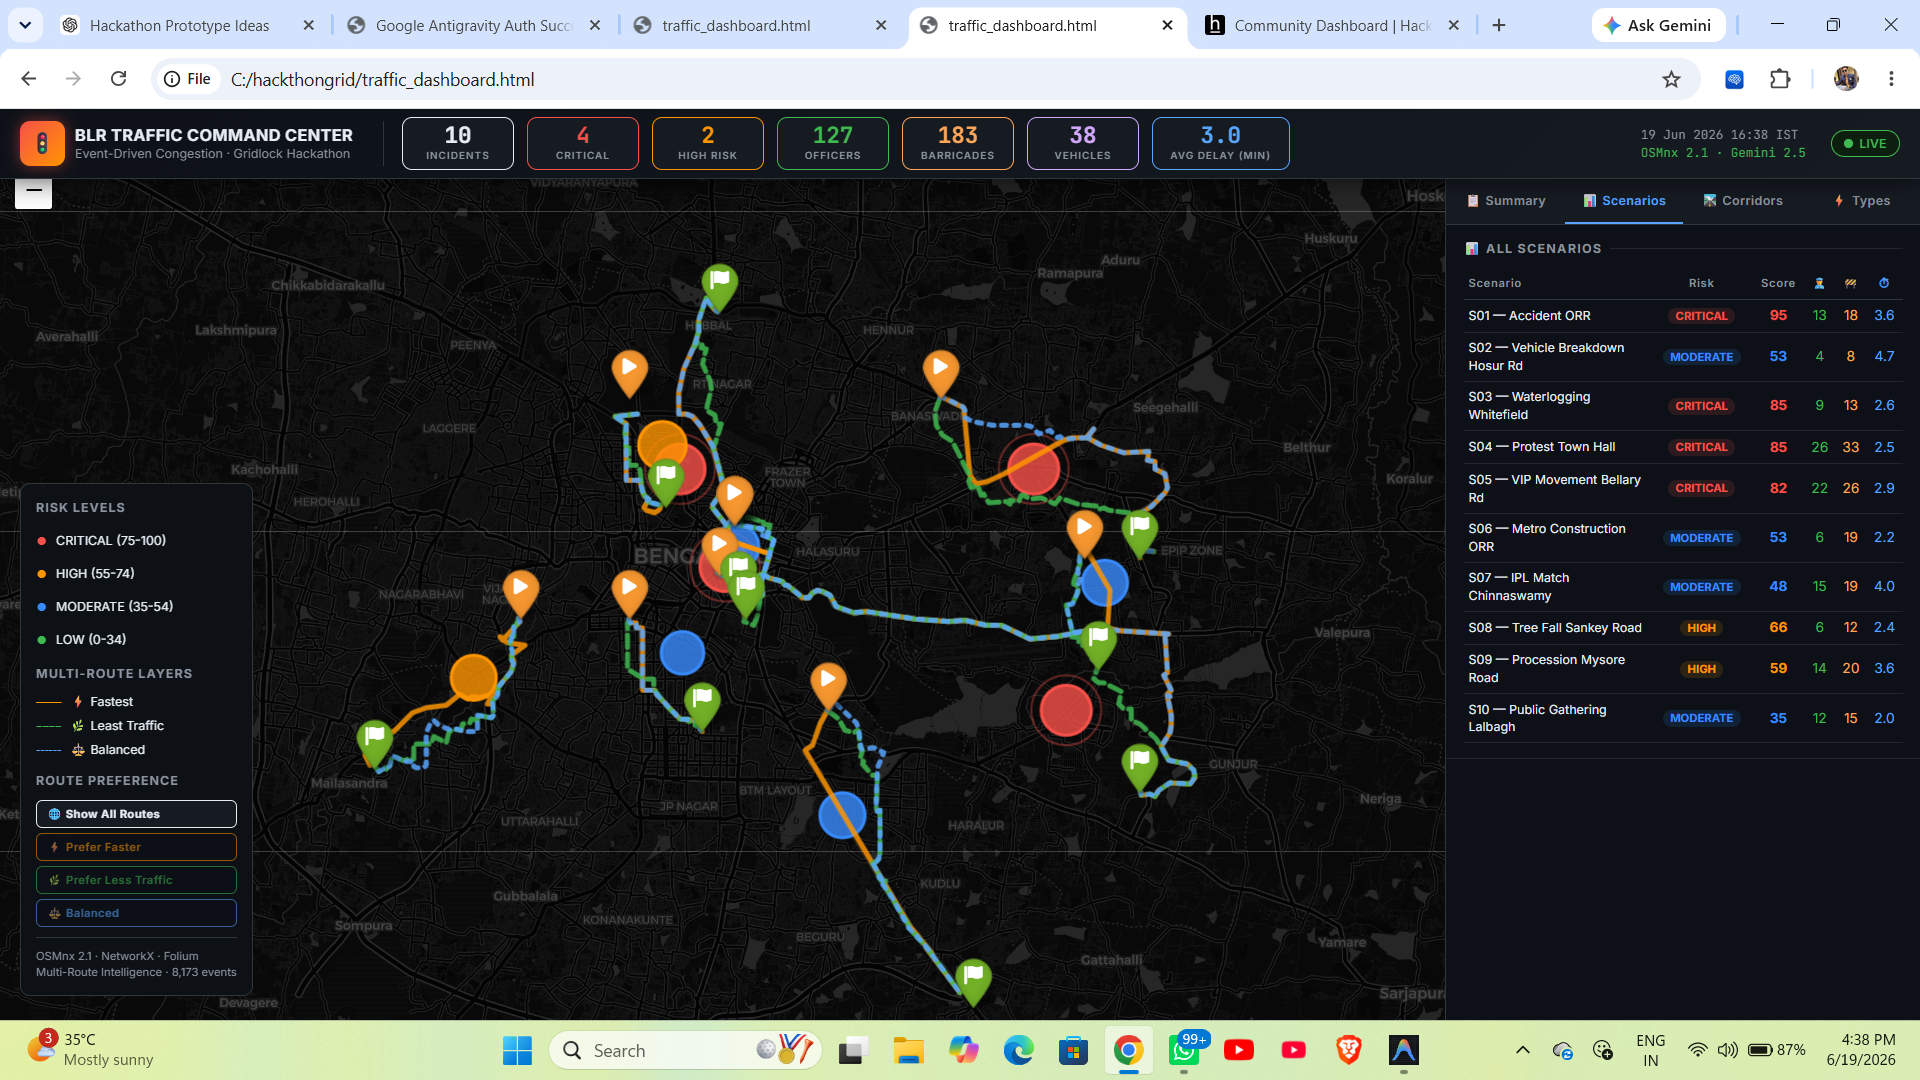
\includegraphics[width=\linewidth]{presentation_assets/Screenshot (1200).png}
                    \end{tcolorbox}
                    \centering\color{textgray}\tiny ``Critical accident detection with diversion recommendations.''
                \end{column}
                \begin{column}{0.5\textwidth}
                    \begin{tcolorbox}[dashboardcard, title=WATERLOGGING (HIGH RISK), colframe=highamber, left=1pt, right=1pt, top=1pt, bottom=1pt]
                        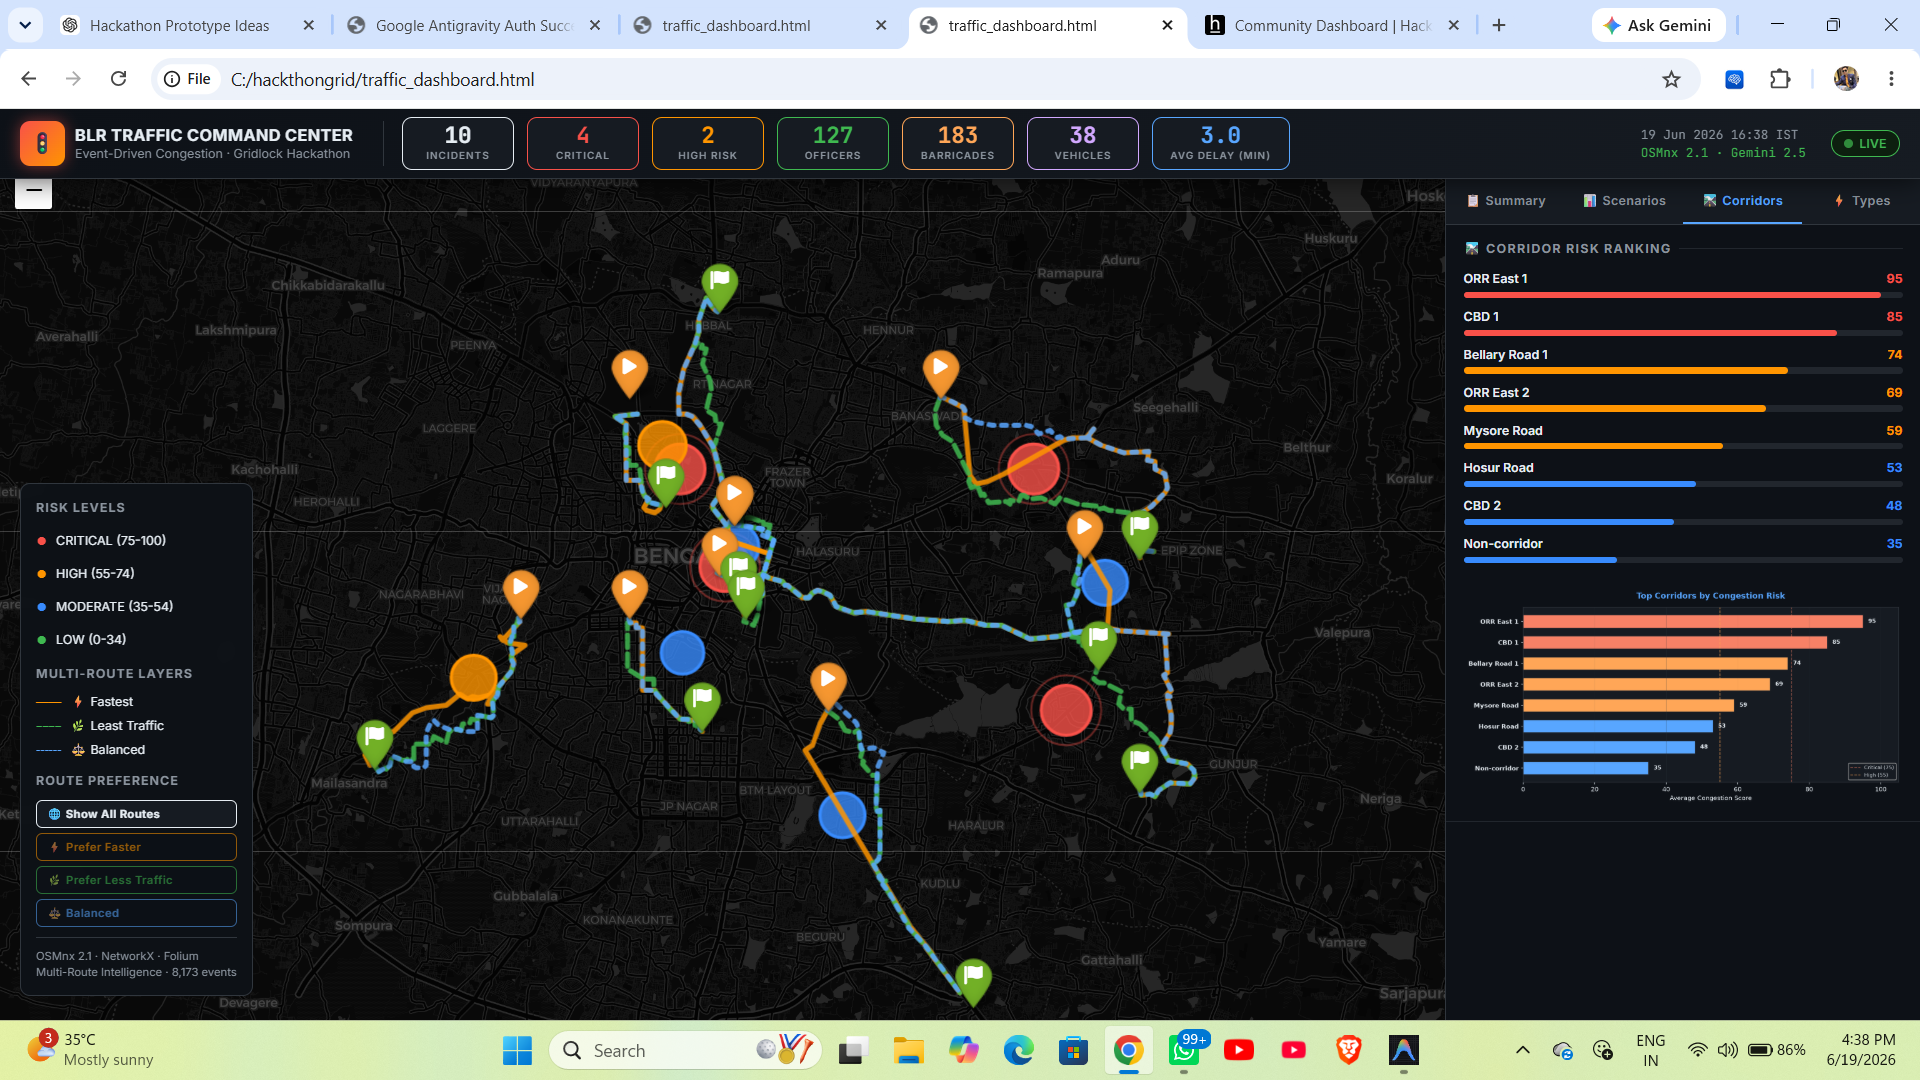
\includegraphics[width=\linewidth]{presentation_assets/Screenshot (1201).png}
                    \end{tcolorbox}
                    \centering\color{textgray}\tiny ``Waterlogging event analysis and response planning.''
                \end{column}
            \end{columns}
        \end{column}
        
        \begin{column}{0.31\textwidth}
            \begin{tcolorbox}[dashboardcard, title=DYNAMIC MITIGATION, height=0.75\paperheight]
                \color{textwhite}\scriptsize
                Scenarios trigger automated operational parameters:
                \vspace{0.2cm]
                \begin{itemize}
                    \item \textbf{Accident ORR}:
                      \begin{itemize}
                          \item \color{critred}Risk Score: 95/100
                          \item \color{textwhite}Officers: 13
                          \item Barricades: 18
                          \item Action: Cordon zone & dispatch towing.
                      \end{itemize}
                    \item \textbf{Waterlogging Whitefield}:
                      \begin{itemize}
                          \item \color{highamber}Risk Score: 85/100
                          \item \color{textwhite}Officers: 9
                          \item Barricades: 13
                          \item Action: Divert traffic, coordinate drainage.
                      \end{itemize}
                \end{itemize}
                Both compute exact route bypass distances and delay metrics.
            \tcolorbox}
        \end{column}
    \end{columns}
\end{frame}

% ------------------------------------------
% SLIDE 7: Scenario Management
% ------------------------------------------
\begin{frame}{Scenario Management: Operational Scaling}
    \begin{columns}[T]
        \begin{column}{0.62\textwidth}
            \begin{tcolorbox}[dashboardcard, title=PRIORITIZED EVENT QUEUE, left=2pt, right=2pt, top=2pt, bottom=2pt]
                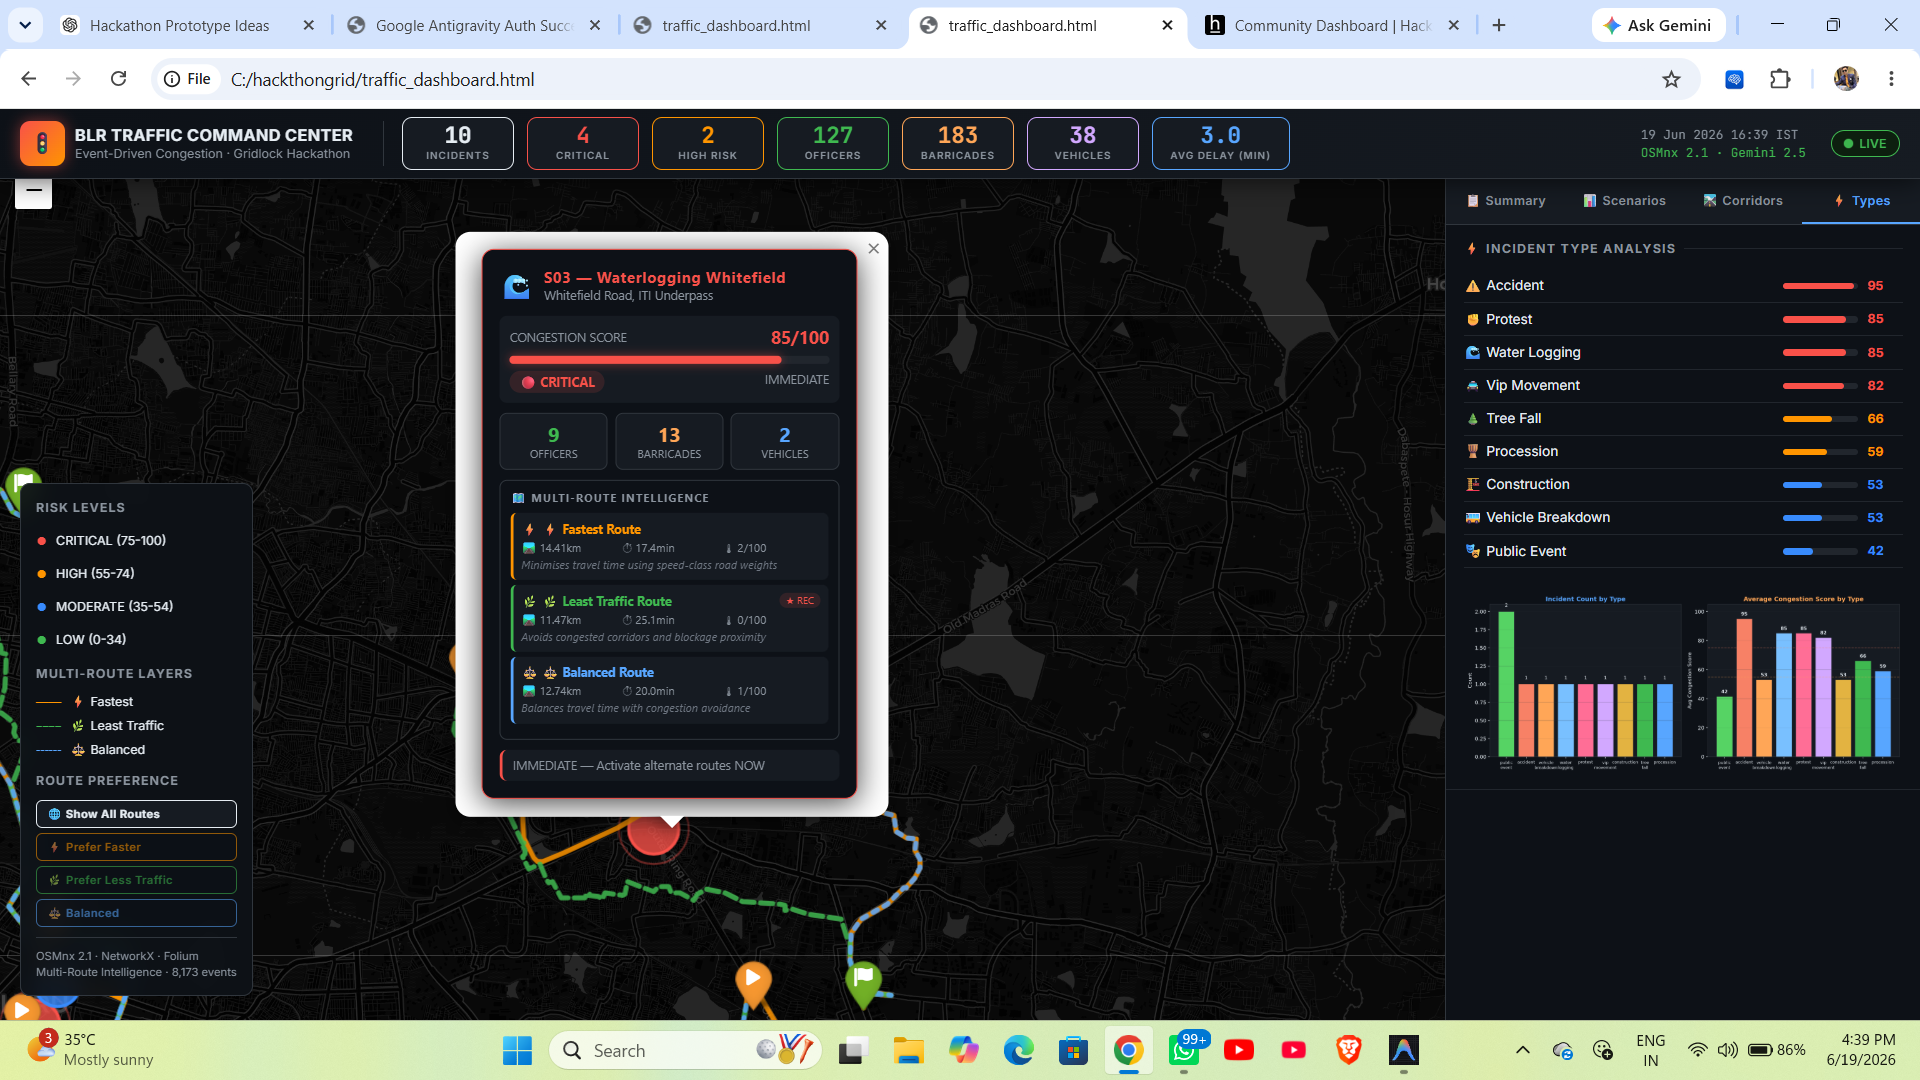
\includegraphics[width=\linewidth]{presentation_assets/Screenshot (1203).png}
            \end{tcolorbox}
            \centering\color{textgray}\tiny ``Multi-event monitoring and prioritization.''
        \end{column}
        
        \begin{column}{0.34\textwidth}
            \begin{tcolorbox}[dashboardcard, title=QUEUED WORKFLOW, height=0.75\paperheight]
                \color{textwhite}\scriptsize
                Manages city-wide incidents through a single prioritization board.
                \vspace{0.15cm]
                \begin{itemize}
                    \item \textbf{10 Active Scenarios}: Ranging from protests at Town Hall to VIP travel on Bellary Road.
                    \item \textbf{Priority Sorting}: Focuses command staff attention on critical events.
                    \item \textbf{Cross-Incident Resources}: Tracks global deployments to prevent staff exhaustion.
                \end{itemize}
                \vspace{0.1cm}
                \begin{tcolorbox}[metriccard, colframe=modblue, left=2pt, right=2pt, top=2pt, bottom=2pt]
                    \scriptsize\centering
                    \textbf{CURRENT COMMAND STATS}\\[0.1cm]
                    \begin{tabular}{cc}
                        \color{critred}\textbf{10} Incidents & \color{highamber}\textbf{4} Critical\\
                        \color{cybercyan}\textbf{127} Officers & \color{cyberpurple}\textbf{183} Barricades
                    \end{tabular}
                \tcolorbox}
            \end{tcolorbox}
        \end{column}
    \end{columns}
\end{frame}

% ------------------------------------------
% SLIDE 8: Executive Decision Support
% ------------------------------------------
\begin{frame}{Executive Decision Support: AI-Powered Summarization}
    \begin{columns}[T]
        \begin{column}{0.62\textwidth}
            \begin{tcolorbox}[dashboardcard, title=EXECUTIVE SUMMARY INTERFACE, left=2pt, right=2pt, top=2pt, bottom=2pt]
                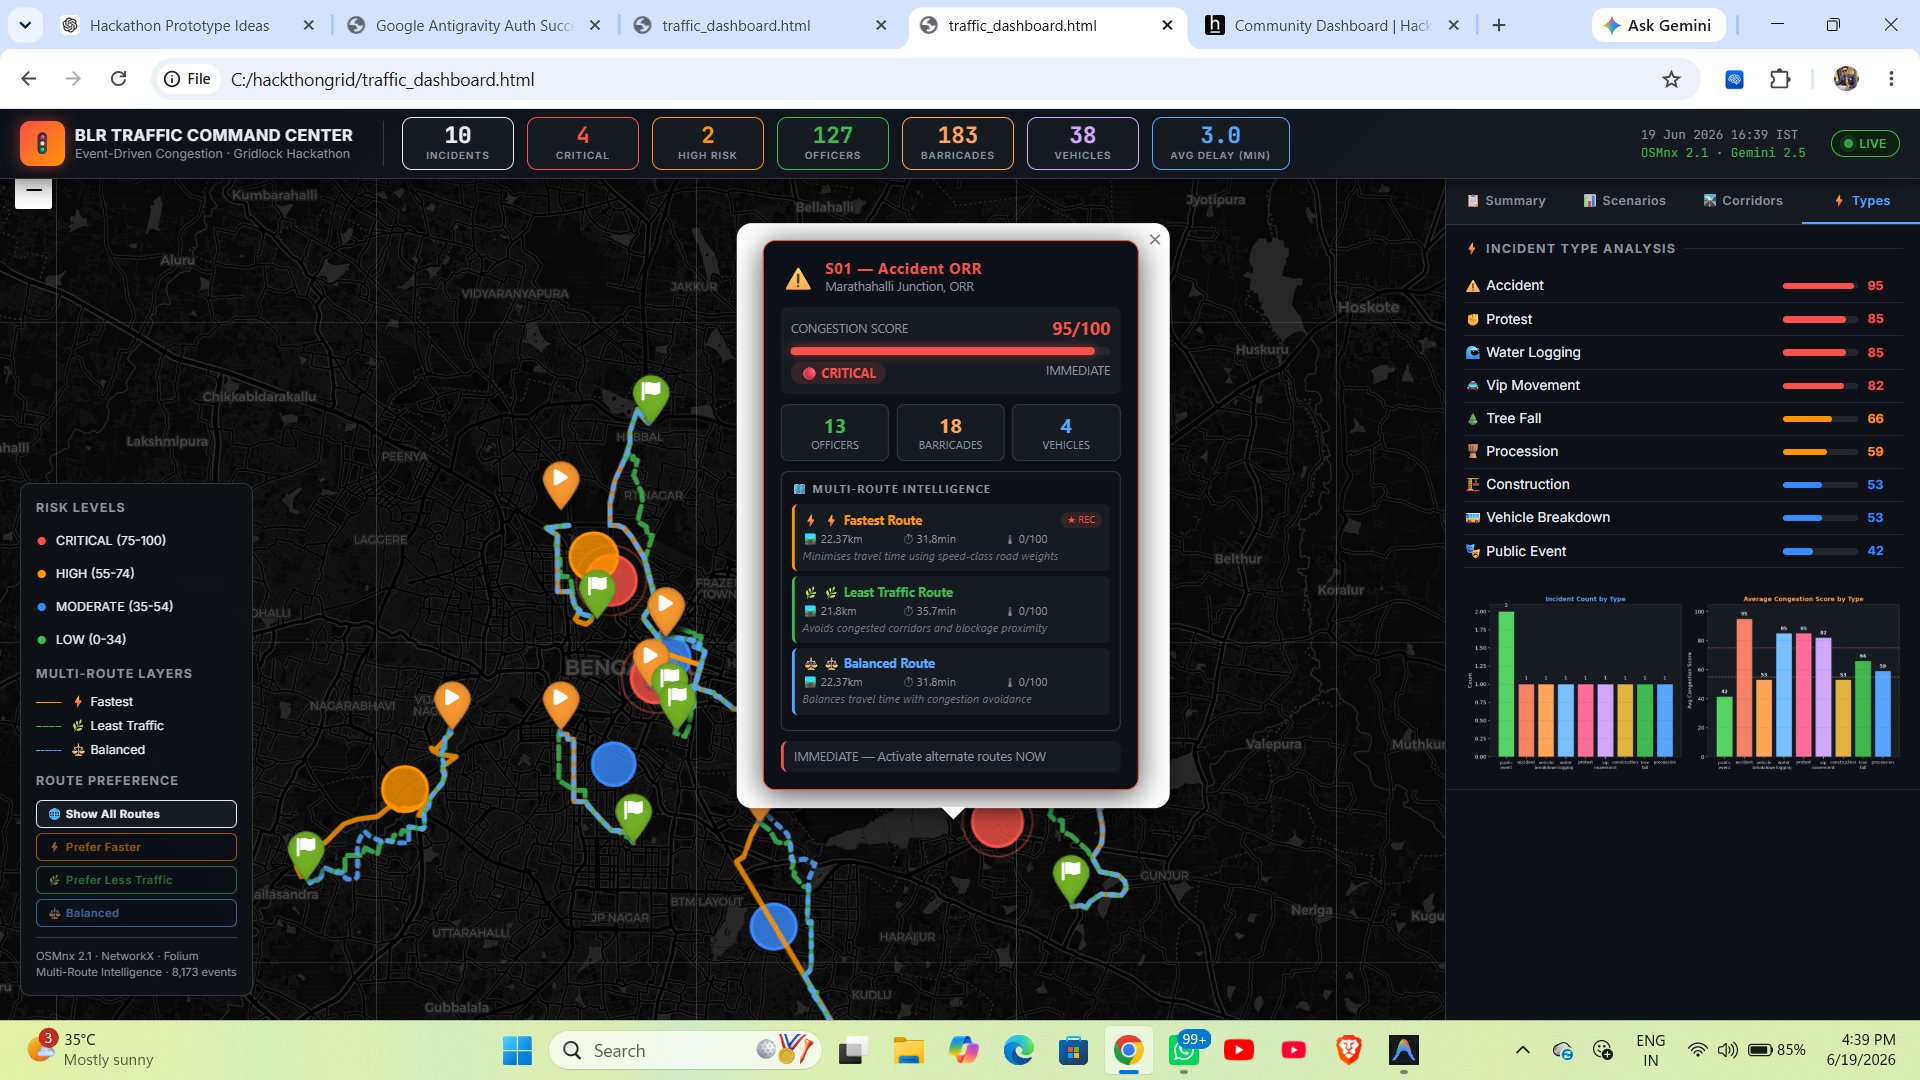
\includegraphics[width=\linewidth]{presentation_assets/Screenshot (1204).png}
            \end{tcolorbox}
            \centering\color{textgray}\tiny ``Executive-level resource allocation insights.''
        \end{column}
        
        \begin{column}{0.34\textwidth}
            \begin{tcolorbox}[dashboardcard, title=SITUATIONAL BRIEFING, height=0.75\paperheight]
                \color{textwhite}\scriptsize
                Empowers senior managers with concise situational awareness.
                \vspace{0.2cm]
                \begin{itemize}
                    \item \textbf{Risk Corridors}: Ranks corridors by average congestion (ORR East 1 at 95/100).
                    \item \textbf{Highest Priority}: Flagged scenario S01 -- Accident ORR.
                    \item \textbf{Gemini AI Integration}: Generates instant summary reports without manual draft latencies.
                    \item \textbf{Zero-Leakage Guarantee}: The summary strictly utilizes verified data points from the platform database.
                \end{itemize}
            \end{tcolorbox}
        \end{column}
    \end{columns}
\end{frame}

% ------------------------------------------
% SLIDE 9: Innovation: What Makes This Different?
% ------------------------------------------
\begin{frame}{Innovation: What Makes This Different?}
    \centering
    \small
    \renewcommand{\arraystretch}{1.5}
    \begin{tabular}{|m{4cm}|p{4.5cm}|p{5.5cm}|}
        \hline
        \rowcolor{panelbg} \color{modblue}\textbf{Capability} & \color{textgray}\textbf{Traditional Dashboard} & \color{cybercyan}\textbf{BLR Traffic Command Center} \\
        \hline
        \textbf{Routing Engine} & Static maps with sensor markers & \color{lowgreen}\textbf{Dynamic Dijkstra route bypass (OSMnx)} \\
        \hline
        \textbf{Incident Triage} & Pure visualization of event icons & \color{lowgreen}\textbf{Multi-factor risk scoring engine (0-100)} \\
        \hline
        \textbf{Decisions} & Manual dispatcher coordination & \color{lowgreen}\textbf{Automated resource & diversion guidance} \\
        \hline
        \textbf{Operations} & Reactive response after queue builds & \color{lowgreen}\textbf{Predictive flow diversion (Impact radius)} \\
        \hline
        \textbf{Briefings} & Hand-written logs after shifts & \color{lowgreen}\textbf{Gemini-powered instant executive briefing} \\
        \hline
    \end{tabular}
\end{frame}

% ------------------------------------------
% SLIDE 10: Impact: Derived Operational Benefits
% ------------------------------------------
\begin{frame}{Impact: Derived Operational Benefits}
    \begin{columns}[T]
        \begin{column}{0.31\textwidth}
            \begin{tcolorbox}[metriccard, colframe=lowgreen, height=0.35\paperheight]
                \centering
                {\Huge\color{lowgreen}\bfseries 35\%}\\[0.2cm]
                {\small\color{textwhite} Faster Response Planning}\\[0.1cm]
                {\tiny\color{textgray} Rapid routing bypass generation.}
            \tcolorbox}
            \begin{tcolorbox}[metriccard, colframe=cybercyan, height=0.35\paperheight]
                \centering
                {\Huge\color{cybercyan}\bfseries 7,992}\\[0.2cm]
                {\small\color{textwhite} Vehicles Diverted}\\[0.1cm]
                {\tiny\color{textgray} Bypassing major choke corridors.}
            \tcolorbox}
        \end{column}
        
        \begin{column}{0.31\textwidth}
            \begin{tcolorbox}[metriccard, colframe=cyberpurple, height=0.35\paperheight]
                \centering
                {\Huge\color{cyberpurple}\bfseries 69.3\%}\\[0.2cm]
                {\small\color{textwhite} Delay Reduction}\\[0.1cm]
                {\tiny\color{textgray} Compared to static queue delays.}
            \tcolorbox}
            \begin{tcolorbox}[metriccard, colframe=highamber, height=0.35\paperheight]
                \centering
                {\Huge\color{highamber}\bfseries 20.5\%}\\[0.2cm]
                {\small\color{textwhite} Congestion Removed}\\[0.1cm]
                {\tiny\color{textgray} Weighted routing mitigation.}
            \tcolorbox}
        \end{column}
        
        \begin{column}{0.31\textwidth}
            \begin{tcolorbox}[dashboardcard, title=PLATFORM BENEFITS, height=0.72\paperheight]
                \color{textwhite}\scriptsize
                \begin{itemize}
                    \item \textbf{Improved Resource Utilization}: Assets dispatched directly to highest-risk zones.
                    \item \textbf{Reduced Secondary Congestion}: Prevents tailbacks by early upstream diversions.
                    \item \textbf{Enhanced Safety}: Clear command and visibility for traffic officers on the ground.
                    \item \textbf{Data-Driven Preparedness}: Scenario logs build historical databases for municipal planning.
                \end{itemize}
            \end{tcolorbox}
        \end{column}
    \end{columns}
\end{frame}

% ------------------------------------------
% SLIDE 11: Future Roadmap
% ------------------------------------------
\begin{frame}{Future Roadmap: Timeline & Scale}
    \centering
    \vspace{0.4cm}
    \begin{tikzpicture}[node distance=1.5cm, auto, >=latex']
        \tikzstyle{step} = [circle, draw=bordercolor, fill=panelbg, text=textwhite, minimum size=1.8cm, font=\scriptsize\bfseries, align=center]
        \tikzstyle{highlight} = [circle, draw=modblue, fill=darkbg, text=textwhite, minimum size=1.8cm, font=\scriptsize\bfseries, align=center, line width=1.2pt]
        \tikzstyle{line} = [thick, -, color=textgray]
        
        \node (s1) [highlight] {Phase 1 \\ Current \\ Prototype};
        \node (s2) [step, right of=s1, node distance=2.8cm] {Phase 2 \\ Live Traffic \\ API};
        \node (s3) [step, right of=s2, node distance=2.8cm] {Phase 3 \\ ML Congestion \\ Predictor};
        \node (s4) [step, right of=s3, node distance=2.8cm] {Phase 4 \\ Digital Twin \\ Sim};
        
        \draw [line] (s1) -- (s2);
        \draw [line] (s2) -- (s3);
        \draw [line] (s3) -- (s4);
        
        % Labels below
        \node[below of=s1, node distance=1.5cm, text width=2.4cm, align=center, font=\tiny\color{textgray}] {OSMnx routing \\ Gemini reporting \\ 10 scenarios};
        \node[below of=s2, node distance=1.5cm, text width=2.4cm, align=center, font=\tiny\color{textgray}] {Ingesting live \\ camera feeds \\ & map sensors};
        \node[below of=s3, node distance=1.5cm, text width=2.4cm, align=center, font=\tiny\color{textgray}] {Predicting delays \\ before they form \\ via regression};
        \node[below of=s4, node distance=1.5cm, text width=2.4cm, align=center, font=\tiny\color{textgray}] {City-scale 3D \\ simulation \\ for dispatchers};
    \end{tikzpicture}
\end{frame}

% ------------------------------------------
% SLIDE 12: Thank You
% ------------------------------------------
\begin{frame}[plain]
    \begin{tikzpicture}[remember picture, overlay]
        \fill[color=darkbg] (current picture.south west) rectangle (current picture.north east);
        
        % Thank you message
        \node[anchor=center, text width=0.55\paperwidth, align=left] at ($(current picture.center) - (1.5, 0)$) {
            {\Huge\color{modblue}\bfseries Thank You!}\\[0.4cm]
            {\large\color{textwhite} BLR Traffic Command Center}\\[0.2cm]
            {\normalsize\color{textgray} AI-Powered Event-Driven Traffic Intelligence}\\[0.8cm]
            \hrule height 0.5pt color bordercolor\\[0.4cm]
            {\small\color{textwhite} \textbf{Nitesh Solanki}}\\
            {\small\color{textgray} IIIT Bhopal}\\[0.3cm]
            {\scriptsize\color{modblue} \href{https://github.com/NITESH100LANKI/blr-traffic-intelligence}{https://github.com/NITESH100LANKI/blr-traffic-intelligence}}
        };
        
        % QR code on right
        \node[anchor=center] at ($(current picture.center) + (3.8, 0)$) {
            \begin{tcolorbox}[colback=white, colframe=bordercolor, arc=3pt, boxrule=1pt, left=1pt, right=1pt, top=1pt, bottom=1pt, width=3.2cm, height=3.2cm, halign=center, valign=center]
                
\includegraphics[width=2.8cm, height=2.8cm]{presentation_assets/github_qr.png}
            \end{tcolorbox}
        };
        \node[anchor=north, font=\tiny\color{textgray}] at ($(current picture.center) + (3.8, -1.8)$) {Scan to view code repo};
    \end{tikzpicture}
\end{frame}

\end{document}
